\section{Descripción TAMA}

En \cite{KOU2008} se introdujo un método novedoso para el análisis del \entrainment acústico/prosódico. Esta técnica consiste, a grandes rasgos, en armar dos series de tiempo para cada uno de los interlocutores y luego utilizar herramientes de análisis sobre las series construídas. Una serie de tiempo, en términos coloquiales, es una colección cronológica de observaciones, como pueden ser los valores de las acciones de una empresa a lo largo del tiempo, o la cantidad de lluvia medida en \emph{ml} para cada mes de cierto año. En el apéndice \ref{sec:time_series} describimos más en detalle los conceptos básicos sobre series de tiempo.

Un problema que resuelve esta técnica es el del alineamiento: si intentásemos comparar cada segmento del habla (utterance) con otros, ¿cómo los alineamos? Una posibilidad sería uno a uno, aunque ésto es muy simplista y poco representativo de la realidad. Al introducir el concepto de series de tiempo, podemos olvidarnos de los segmentos del habla y simplemente utilizar estas construcciones.

Para construir la serie de tiempo de cada interlocutor debemos, en primer lugar, dividir el diálogo en ventanas solapadas de igual tamaño. A la diferencia entre ventana y ventana llamaremos \emph{frame step}, y al tamaño de ventana \emph{frame length}. Consideraremos sólo los segmentos de habla que se encuentren dentro de cada ventana; aquellos segumentos que atraviesen los límites de las ventanas son cortados para que se mantengan dentro de éste. En la figura \ref{tama} se ilustra el proceso.

\begin{figure}
\centering
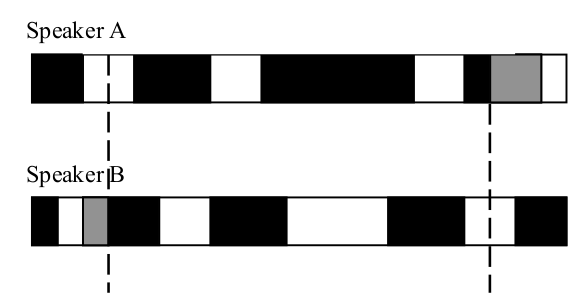
\includegraphics[width=10cm]{images/tama.png}
\caption{Gráfico de la separación del diálogo en ventanas}
\label{tama}
\end{figure}

Nuestro corpus está anotado de manera que tenemos separadas los intervalos donde los interlocutores hablan (llamaremos a cada uno de éstos locuciones o \emph{utterances}). Para cada una de los frames, calcularemos la media

\begin{align}
    \mu &= \sum\limits_{i=1}^N f_i dr_i \label{eq:tama_mean}\\
    dr_i &= \frac{d_i}{\sum\limits_{i=1}^N d_i}
\end{align}

donde $i$ itera sobre las locuciones dentro del \emph{frame}, $d_i$ es la duración de la locución y $f_i$ es el valor de la \emph{feature} que estamos midiendo.

Como se ve en \ref{eq:tama_mean}, el $\mu$ que calculamos es una media ponderada por la duración de las locuciones. Así, por ejemplo, al calcular una serie de tiempo sobre el \emph{pitch}, la contribución de interjecciones (usualmente de alto valor) estará disminuída por su breve duración.

La serie de tiempo constará entonces de la secuencia de medias calculadas con \ref{eq:tama_mean} para cada uno de los frames.


\nota{Mejorar el dibujo éste y agregarle una descripción}
